%% LaTeX-Beamer template for KIT design
%% by Erik Burger, Christian Hammer
%% title picture by Klaus Krogmann
%%
%% version 2.1
%%
%% mostly compatible to KIT corporate design v2.0
%% http://intranet.kit.edu/gestaltungsrichtlinien.php
%%
%% Problems, bugs and comments to
%% burger@kit.edu

\documentclass[18pt]{beamer}
\usepackage[utf8x]{inputenc}
\usepackage{units}
\usepackage{booktabs}

%% CUSTOM
\usepackage{amsmath}
\usepackage{algpseudocode}

%% Definitions
\DeclareMathOperator{\div2}{div}
\renewcommand{\algorithmicrequire}{\textbf{Input:}}
\renewcommand{\algorithmicensure}{\textbf{Output:}}
\algnewcommand\algorithmicto{\textbf{to}}
\algrenewtext{For}[3]{\algorithmicfor\ $#1 \gets #2$ \algorithmicto\ $#3$ \algorithmicdo}
\algnewcommand\algorithmicod{\textbf{od}}
\algrenewtext{EndWhile}{\algorithmicod}
\algrenewtext{EndFor}{\algorithmicod}
%\AtBeginSection[]{%
%\begin{frame}<beamer> % do nothing in handouts
%    \frametitle{Überblick}
%    \tableofcontents[sectionstyle=show/shaded,
%    subsectionstyle=show/show/hide]
%\end{frame}
%}
%\AtBeginSubsection[]{%
%\begin{frame}<beamer> % do nothing in handouts
%    \frametitle{Überblick}
%    \tableofcontents[sectionstyle=show/shaded,
%    subsectionstyle=show/shaded/hide]
%\end{frame}
%}

%% SLIDE FORMAT

% use 'beamerthemekit' for standard 4:3 ratio
% for widescreen slides (16:9), use 'beamerthemekitwide'

\usepackage{templates/beamerthemekit}
%\usepackage{templates/beamerthemekitwide}

 %% TITLE PICTURE

 % if a custom picture is to be used on the title page, copy it into the 'logos'
 % directory, in the line below, replace 'mypicture' with the 
 % filename (without extension) and uncomment the following line
 % (picture proportions: 63 : 20 for standard, 169 : 40 for wide
 % *.eps format if you use latex+dvips+ps2pdf, 
 % *.jpg/*.png/*.pdf if you use pdflatex)


 \titleimage{banner}
 
 
%% Define some colors:
\definecolor{darkblue}{rgb}{0,0,.5}
\definecolor{darkgreen}{rgb}{0,.5,0}

 %% TITLE LOGO

 % for a custom logo on the front page, copy your file into the 'logos'
 % directory, insert the filename in the line below and uncomment it

\titlelogo{logo_150x150}
 
 % (*.eps format if you use latex+dvips+ps2pdf,
 % *.jpg/*.png/*.pdf if you use pdflatex)
 
 %% TikZ INTEGRATION
 
 % use these packages for PCM symbols and UML classes
 % \usepackage{templates/tikzkit}
 % \usepackage{templates/tikzuml}
 
 % the presentation starts here
 
\author{Dominik Muth - dominik.muth@student.kit.edu}
\institute{Institut f\"ur Informatik}

\subtitle{Foliensatz 7}
\date{6. Dezember 2012}

\begin{document}

\begin{frame}
    \titlepage
\end{frame}

\begin{frame}{Outline/Gliederung}
    \tableofcontents
\end{frame}

\section{Übungsblatt 6}
\begin{frame}{Allgemeine Fehler, Fragen}
    \begin{block}{Allgemeines}
        \begin{itemize}
            \item Bei der vollständige Induktion können noch viele Punkte geholt werden
            \item Beweis zu Injektiv und Surjektiv mittels Definitionen
        \end{itemize}
    \end{block}
\end{frame}

\section{Wiederholung}
\begin{frame}{Quickies}
    \begin{itemize}
        \item Die Huffman-Codierung ist präfixfrei. \visible<2->{Wahr} 
        \item Was macht $\Num2_b\left( w \right)$?
        \item Gilt für einen Homomorphismus $h\left( xy \right) = h\left( x \right)\circ h\left( y \right)$? \visible<3->{Wahr}
        \item $\left( y,x \right) \in R$ kann als $yRx$ geschrieben werden.\visible<4->{Wahr.}
    \end{itemize}
\end{frame}

\section{Graphen}
\begin{frame}{Graphen: Definition}
    \begin{block}{Gerichteter Graph}
        Ein Tupel $G = \left( V, E \right)$ mit 
        \begin{itemize}
            \item der nichtleeren \emph{Knotenmenge} $V$ und
            \item der \emph{Kantenmenge} $E\subseteq \left\{ V \times V \right\}$
        \end{itemize}
        nennen wir \emph{gerichteten Graph}.
    \end{block}
    \pause
    \begin{block}{Ungerichteter Graph}
        Ein Tupel $G = \left( V, E \right)$ mit 
        \begin{itemize}
            \item der nichtleeren \emph{Knotenmenge} $V$ und
            \item der \emph{Kantenmenge} $E\subseteq \left\{ \left\{ x, y \right\} \big| x\in V, y\in V \right\}$
        \end{itemize}
        nennen wir \emph{ungerichteten Graph}.
    \end{block}
    \pause
    Wo ist der Unterschied?
\end{frame}
\begin{frame}{Schlingen}
    \begin{block}{Definition}
        Eine Kante mit identischem Start- und Endpunkt nennt man \emph{Schlinge}.
    \end{block}
    Ein Graph ohne Schlinge ist \emph{schlingenfrei}.
\end{frame}
\begin{frame}{Teilgraph}
    \begin{block}{Definition}
        Ein \emph{Teilgraph} $T$ von $G$ ist ein Graph $T = \left( V', E' \right)$, bei dem
        \begin{itemize}
            \item Knoten- und Kantenmenge Teilmengen des Graphen G sind und
            \item deren Kanten nicht aus dem Teilgraph hinausführen.
        \end{itemize}
        \pause
        Formell (hier für gerichtete Graphen):
        \begin{align*}
            V' \subseteq V\\
            E' \subseteq E \cap V' \times V'
        \end{align*}
    \end{block}
\end{frame}
\begin{frame}{Grad}
    \begin{block}{Definition}
        Der Eingangsgrad eines Knoten $k$ ist die Anzahl der Knoten $x$, di emit der Kante zum Knoten $k$ verbunden sind. Also
        \begin{align*}
            d^+\left( k \right) = \big| \left\{ x \big| \left( x,k \right)\in E \right\}\big|
        \end{align*}
        Der Ausgangsgrad wird analog definiert.
    \end{block}
    Analog für Ausgangsgraphen.
    Als ``Grad'' wird die Summe von Eingangs- und Ausgangsknoten bezeichnet.  
\end{frame}
\begin{frame}{Pfad}
    \begin{block}{Definition}
        Ein \emph{Pfad} ist ein möglicher Weg über Knoten und Kanten im Graphen.\\
        Formal: eine nichtleere Liste
        \begin{align*}
            P = \left( v_0,v_1,\dots , v_n \right)\\
            \forall v_i \in P: \left( v_i,v_{i+1} \right) \in E
        \end{align*}
        Der Pfad hat als Länge die Anzahl seiner Kanten.
    \end{block}
\end{frame}
\begin{frame}{Eigenschaften von Pfaden}
    \begin{itemize}
        \item \emph{Geschlossen:} Wenn $v_0 = v_n$ gilt (auch ``Zyklus'')
        \item \emph{Wiederholungsfrei:} Wenn alle Knoten paarweise verschieden sind (außer erster und letzter Knoten)
        \item \emph{Einfacher Zyklus:} Wenn er geschlossen und wiederholungsfrei ist.
    \end{itemize}
\end{frame}

\begin{frame}{Quickies}
    \begin{itemize}
        \item Wieviel Kanten kann ein gerichteter Graph maximal haben, wenn Schlingen erlaubt sind?\visible<2->{$n^2$}
        \item Wieviele kanten kann ein gerichteter Graph maximal haben, wenn er schlingenfrei ist?\visible<3->{n\left( n-1 \right)}
    \end{itemize}
\end{frame}

\begin{frame}{Eigenschaften von Graphen}
    \begin{block}{Isomorphie}
        Ein Graph $G_1 = \left( V_1, e_1 \right) $ heißt \emph{isomorph} zu einem Graphen $G_2 = \left( V_2,E_s \right)$, wenn es eine bijektive Abbildung $f: V_1 \rightarrow V_2$ gibt mit der Eigenschaft:
        \begin{align*}
            \forall x\in V_1: \forall y \in V_1: \left( x, y \right) \in E_1 \Longleftrightarrow \left( f\left( x \right),f\left( y \right) \right)\in E_2
        \end{align*}
    \end{block}
    Und was heißt das? \visible<2->{Durch Umbenenung der Knoten.}\\
    \pause
    Das ist eine Relation. Welche Eigenschaften hat sie?
    \visible<3->{\begin{itemize}
        \item Isomorphie ist reflexiv
        \item Isomorphie ist transitiv
        \item Isomorphie ist symmetrisch
    \end{itemize}}
\end{frame}

\begin{frame}{Quickie}
    Für welche der folgenden sechs Graphen gibt es einen Isomorphismus zu einem der anderen fünf Graphen? Geben Sie jeweils den zugehörigen Isomorphismus an.
    \begin{figure}[h]
        \centering
        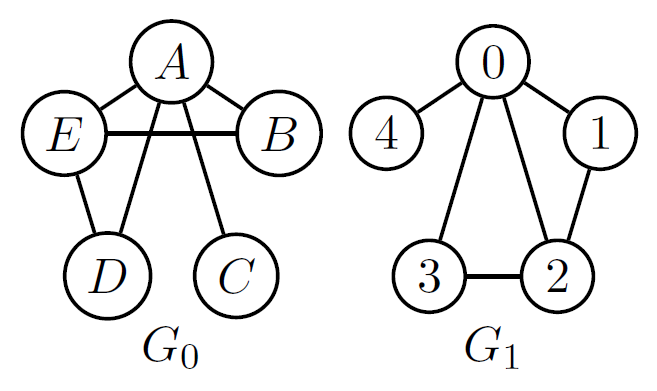
\includegraphics[width=\textwidth,height=\textheight,keepaspectratio]{graphics/07/isomorphie.png}
    \end{figure}
\end{frame}

\begin{frame}{Produkt von Kanten}
    $E$ sei die Kantenmenge eines Graphen $G = \left( V,E \right)$. Was ist $E \circ E$?
    \pause
    \begin{align*}
        E^2 = E\circ E = \left\{ \left( x,z \right)\in V\times V\big| \exists y \in V: \left( x,y \right)\in E \wedge \left( y,z \right) \in E \right\}
    \end{align*}
    In der Menge $E^2$ sind also alle Pfade der Länge $2$. Sonderfall $E^0$ - dort sind alle Schleifen. Es gilt:
    \begin{block}{Produkt von Kanten}
        Ein Paar von Knoten $\left( x,y \right)$ ist genau dann in der Relation $E^i$, wenn $x$ und $y$ in $G$ durch einen Pfad der Länge $i$ miteinander verbunden sind.
    \end{block}
    \pause
    Was ist $E^*$?
\end{frame}

\begin{frame}{Quickies}
    \begin{itemize}
        \item Wieviele Kanten kann ein ungerichteter Graph maximal haben, wenn er schlingenfrei ist? \visible<2->{$\frac{n\left( n-1 \right)}{2}$}
        \item Wieviele Kanten kann ein ungerichteter Graph maximal haben, wenn er Schlingen haben darf? \visible<3->{$\frac{n\left( n+1 \right)}{2}$}
    \end{itemize}
\end{frame}

\section{Aufgaben}
\begin{frame}{Winter 08/09}
    \begin{itemize}
        \item Zeichnen Sie alle möglichen gerichteten Bäume mit genau vier Knoten, von denen keine zwei isomorph sind.
        \item Zeichnen Sie alle möglichen ungerichteten Bäume mit genau fünf Knoten, von denen keine zwei Isomorph sind.
    \end{itemize}
\end{frame}

\begin{frame}{Winter 08/09}
    Gegeben sei der Graph $G=(V, E)$ mit $V=\{0, 1\}^3$ und $E=\{(xw, wy) \mid x, y \in \{0, 1\} \land w \in \{0, 1\}^2\}$.
    \begin{enumerate}
        \item Zeichnen Sie den Graphen
        \item Geben Sie einen Zyklus in $G$ an, der außer dem Anfangs- und Endknoten jeden Knoten von $G$ genau einmal enthält.
        \item Geben Sie einen geschlossenen Pfad in $G$ an, der jede Kante von $G$ genau einmal enthält.
    \end{enumerate}
\end{frame}

\begin{frame}{Winter 10/11}
    Sei $T_1 = \left( V_1, E_1 \right)$ ein gerichteter Baum mit Wurzel $r_1$, $T_2 = \left( V_2, E_2 \right)$ ein gerichteter Baum mit Wurzel $r_2$ und es gelte $V_1 \cap V_2 = \left\{  \right\}$. Sei $r \notin V_1 \cup V_2 $.\\
    Zeigen Sie:
    \begin{align*}
        T_1 \circ_r T_2 = \left( V_1 \cup V_2 \cup r, E_1 \cup E_2 \cup \left\{ \left( r, r_1 \right),\left( r,r_2 \right) \right\} \right)
    \end{align*}
    ist ein gerichteter Baum mit Wurzel r.
\end{frame}
\end{document}
